\section{Batch Logging}

In serial logging, all transactions must obtain an unique and monotonically increasing LSN from the global LSN variable. This become problematic when there are many transactions occurring at the same time because they all access the same variable and thus create a bottleneck. In batch logging, this problem is solved by having multiple loggers with their individual and independent local LSNs. Transactions are evenly distributed to the loggers and each transaction can now take their LSN from the local LSN of their respective loggers. This eliminates the need for a global LSN and thus removes its inherent bottleneck.
\begin{figure}[h]
\caption{Serial logging versus Batch logging}
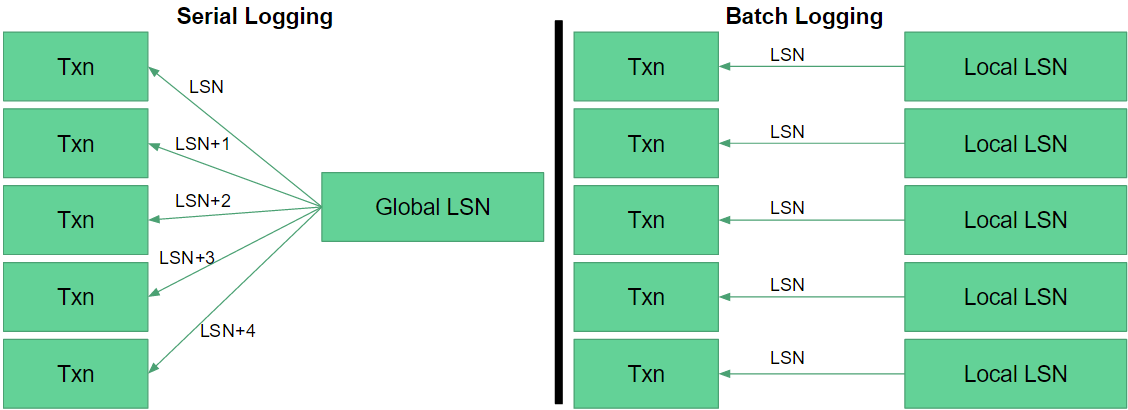
\includegraphics[width=\textwidth]{SerialvsBatch.png}
\end{figure}
With multiple local loggers and their local LSNs, it must be assumed that there are dependencies between the loggers because it cannot be determined otherwise due to the lack of a global serial order, as was present in serial logging with the global LSN. This means that all loggers must sync after a certain interval before they can return to the user, causing a increase in latency compared to serial logging.

In our implementation, we handle the syncing of loggers by flushing all log buffers to disk as soon as one becomes full. A bit vector is used to communicate between the loggers, where the index of the bit corresponds to the number of the logger and the logger flushes if its bit is 1. When a logger fills up its buffer, it changes all bits of the vector to be 1 to signal all other loggers to flush their buffers too. Each logger checks the bit vector upon receiving a transaction, and if their respective bit is 1, then the logger flushes  and toggles its bit to 0 before placing the newly received transaction into its buffer. 

